\documentclass[11pt]{article}
\usepackage[letterpaper,margin=1in]{geometry}
\usepackage{amsmath,amssymb,amsthm}
\usepackage{graphicx}
\usepackage{booktabs}
\usepackage{caption}
\usepackage{subcaption}
\usepackage{enumitem}
\usepackage{titlesec}
\usepackage{fancyhdr}
\usepackage{placeins}
\usepackage{float}
\usepackage{xcolor}
\PassOptionsToPackage{hyphens}{url}
\usepackage[hidelinks]{hyperref}
\setlength{\parskip}{0.4em}
\setlength{\parindent}{0pt}
\setlength{\emergencystretch}{2em}
\titleformat{\section}{\large\bfseries}{\thesection.}{0.6em}{}
\titlespacing*{\section}{0pt}{1.4em}{0.5em}
\titleformat{\subsection}{\normalsize\bfseries}{\thesubsection}{0.5em}{}
\titlespacing*{\subsection}{0pt}{1.0em}{0.3em}
\captionsetup{font=small,labelfont=bf,labelsep=period,skip=6pt}
\setlist[itemize]{leftmargin=1.3em,itemsep=2pt,topsep=3pt,parsep=0pt}
\setlist[enumerate]{leftmargin=1.6em,itemsep=2pt,topsep=3pt,parsep=0pt}
\pagestyle{fancy}
\fancyhf{}
\fancyhead[L]{\small CS 6362: Advanced Machine Learning}
\fancyhead[R]{\small Assignment 2 \,\textbar\, Bibek Dhungana}
\fancyfoot[C]{\small\thepage}
\renewcommand{\headrulewidth}{0.4pt}
\newcommand{\code}[1]{\texttt{#1}}
\newcommand{\repo}[1]{\nolinkurl{#1}}   % repository names, may break at / and -
\newcommand{\E}{\mathbb{E}}
\newcommand{\R}{\mathbb{R}}
\newcommand{\KL}[2]{D_{\mathrm{KL}}\!\left(#1\,\|\,#2\right)}
\newcommand{\TODO}[1]{\textcolor{red}{[#1]}}
\newtheorem{theorem}{Theorem}

\begin{document}
\begin{center}
  {\LARGE\bfseries Paper 1: Understanding deep learning requires\\[2pt] rethinking generalization}\\[5pt]
  {\large Zhang, Bengio, Hardt, Recht, Vinyals (ICLR 2017)}\\[4pt]
  Bibek Dhungana \quad\textbar\quad CS 6362 Assignment 2 \quad\textbar\quad \today
\end{center}

\section{Problem statement and summary}

\subsection{Setup}
The training set $S=\{(x_i,y_i)\}_{i=1}^n$ is drawn i.i.d.\ from an unknown distribution $\mathcal D$, with images $x_i\in\R^d$ and labels $y_i\in\{1,\dots,k\}$. For CIFAR-10 in the paper, $n=50{,}000$, $k=10$ and $d=28\cdot28\cdot3=2352$ after cropping. A network $f_\theta:\R^d\to\R^k$ outputs one score per class. For a loss $\ell$ (cross entropy in training, 0--1 loss for reported errors), the empirical training risk and population risk are
\[
  \hat R_n(\theta)=\frac1n\sum_{i=1}^n \ell\big(f_\theta(x_i),y_i\big),\qquad
  R(\theta)=\E_{(x,y)\sim\mathcal D}\,\ell\big(f_\theta(x),y\big),
\]
and the generalization gap is $R(\theta)-\hat R_n(\theta)$. $R$ is estimated on the 10{,}000 test images.

The puzzle is that these networks have up to 1.6 million weights for 50{,}000 images, reach zero training classification error, and still have low test error. To state a capacity bound precisely, let $\mathcal H$ be a class of loss functions $h:(x,y)\mapsto[0,1]$, such as classification errors. Its empirical Rademacher complexity is
\[
  \hat{\mathfrak R}_n(\mathcal H)=\E_{\sigma}\Big[\sup_{h\in\mathcal H}\frac1n\sum_{i=1}^n\sigma_i\,h(x_i,y_i)\Big],
\]
where the $\sigma_i\in\{-1,+1\}$ are independent fair coin flips. With probability at least $1-\delta$, every $h\in\mathcal H$ satisfies $R(h)\le\hat R_n(h)+2\,\hat{\mathfrak R}_n(\mathcal H)+O\big(\sqrt{\log(1/\delta)/n}\big)$. $\hat{\mathfrak R}_n$ measures how well $\mathcal H$ can fit random labels on the training inputs and never uses the true labels. If the classifier can realize every binary labeling, its $\{-1,+1\}$ prediction class has empirical complexity 1 and its 0--1 loss class has complexity $1/2$. The resulting bound is vacuous. This bounded-loss statement does not apply directly to unbounded cross entropy.

\subsection{Method}
The paper's tool is a randomization test. A standard network is trained with its usual hyper-parameters on CIFAR-10, and again on copies where the signal is destroyed: labels partially corrupted (each one replaced with probability $p$ by a class drawn uniformly from all $k$) or completely random ($p=1$), pixels shuffled by one fixed permutation (\emph{shuffled pixels}) or by a new permutation for each image (\emph{random pixels}), or images replaced by Gaussian noise with the same mean and variance.

The networks fit the randomized training sets with a moderate slowdown, and fully random labels give test error near 90\% (Figure~1). Fitting sampled random labelings is evidence of large capacity, although it does not prove that every labeling can be fit. Bounds based only on worst-case class capacity, or a uniform stability estimate that does not distinguish these data, can be too loose to explain the difference between the true-label and random-label runs. The explanation has to involve the data and the training algorithm.

\emph{Explicit regularization is not the main reason}: Inception gets 85.75\% test accuracy with no regularizer and 89.05\% with cropping and weight decay, and it still fits random labels with weight decay on. \emph{Memorizing is cheap} (Theorem~1): a two-layer ReLU network with $2n+d$ weights, about 102{,}000 for CIFAR-10, can fit any labels on $n$ points. So the surprise is not that the networks \emph{can} represent random labels, but that SGD \emph{finds} such a solution. \emph{SGD has an implicit bias} in the linear case (Section~5). Run SGD on $f(x)=\langle w,x\rangle$ from $w_0=0$. Each update adds a multiple of some $x_i$, so $w=X^\top\alpha$ for some $\alpha\in\R^n$, where $X\in\R^{n\times d}$ stacks the inputs. If $w$ fits the data and $XX^\top$ is invertible (which needs $n\le d$),
\[
  Xw=y \;\Rightarrow\; XX^\top\alpha=y \;\Rightarrow\; w=X^\top(XX^\top)^{-1}y,
\]
which is the minimum-norm solution of $Xw=y$. SGD picks the smallest-norm interpolant without being asked to. The authors admit this is only part of the story: on MNIST the norm does not predict the test error (wavelet preprocessing raises it from 220 to 390 but halves the error).

\subsection{Answers to the questions in the assignment}
\textbf{How are random labels generated across epochs, and what would go wrong otherwise?} They are drawn once before training and reused in every epoch (``fixed and consistent across epochs'' in the paper). If a new label were drawn each time an image is seen, the labels would be pure noise. The best prediction would then be the uniform distribution, the minimum expected cross entropy would be $\log 10\approx2.30$, and there would be nothing to memorize, so the experiment would say nothing about capacity.

\textbf{With corruption probability $p$, what fraction of labels differs from the truth, and what test error should we expect at $p=1$?} A label changes when it is picked (probability $p$) and the new class differs from the old one (probability $1-1/k$), so the fraction is $p(1-1/k)=0.9p$. My runs had 0.179, 0.357, 0.540, 0.720 and 0.899 for $p=0.2,\dots,1.0$. At $p=1$, independently randomized test labels give expected error $1-1/k=0.9$ for any classifier. On clean test labels, 90\% is the chance baseline expected when no class signal has been learned; randomizing only the training labels does not force every fitted classifier to attain exactly that error.

\textbf{What optimizer, learning-rate schedule, preprocessing and regularization do the authors use?} From Appendix~A: pixels are divided by 255, center-cropped to $28\times28$, and each image is whitened separately (subtract its mean, divide by its standard deviation). The optimizer is SGD with momentum 0.9. The learning rate starts at 0.1 for Inception and 0.01 for AlexNet and the MLPs, and is multiplied by 0.95 after every epoch. The randomization experiments use no weight decay, dropout or data augmentation. The batch size is not given.

\section{Reproduction of Figure 1}

\subsection{LLM, conversation and code}
\begin{itemize}
  \item \textbf{LLM:} ChatGPT (GPT-5.6) for the main conversation. I also asked Claude and Gemini some side questions to understand concepts related to the paper.
  \item \textbf{Shared conversation}:\newline \url{https://chatgpt.com/share/e/6ad70878-aa80-83e9-a81a-71775854baf0}
  \item \textbf{Code:} folder \repo{paper1:Rethinking-Generalization/code} of\newline \url{https://github.com/dhunganabibek/reading-and-reproducing-papers}. The notebook \code{reproduce\_fig1.ipynb} redraws the figure and prints every number in this report from the saved logs.
  \item I did not give the LLM any existing implementation before the Phase~3 snapshot, which I saved on 10 October 2026.
\end{itemize}

\subsection{Setup and choices}
\begin{table}[H]\centering\small
  \begin{tabular}{@{}l@{\quad}p{0.76\textwidth}@{}}
    \toprule
    Data & CIFAR-10, 50{,}000 train / 10{,}000 test, center crop to $28\times28$, per-image whitening\\
    Networks & small Inception, small AlexNet, MLP with one hidden layer of 512 units; 1{,}649{,}402 / 1{,}387{,}786 / 1{,}209{,}866 parameters\\
    Optimizer & SGD, momentum 0.9, learning rate 0.1 (Inception) or 0.01 (others), times 0.95 every epoch; no regularization\\
    Batch size & 128; not stated in the paper, but the spacing of the points in its Figure~1a matches (Section~\ref{sec:mismatch})\\
    Stopping & at 100\% training accuracy, or after 100 epochs\\
    Corruption & $p=0,\,0.2,\,0.4,\,0.6,\,0.8,\,1.0$\\
    Random pixels & all 2352 values of an image permuted; a second run keeps the color values of each pixel together\\
    Seeds & one run per setting\\
    \bottomrule
  \end{tabular}
  \caption{Setup of my runs.}
  \label{tab:setup}
\end{table}

\textbf{Convergence time (Figure 1b).} The paper never defines ``time to overfit''. I use the number of SGD steps until the accuracy on the whole training set, checked after every epoch, first reaches 99\%. A 100\% threshold does not work, because the MLP stalls at 99.2--99.97\% once the learning rate has decayed. The paper's own Table~1 shows the same thing on random labels (99.34\% for this MLP, 99.82\% for AlexNet).

\textbf{Reduced grid.} I ran all three networks but only 6 of the paper's 11 corruption levels, which kept the Inception sweep to about three GPU hours on my laptop.

\begin{figure}[t]\centering
  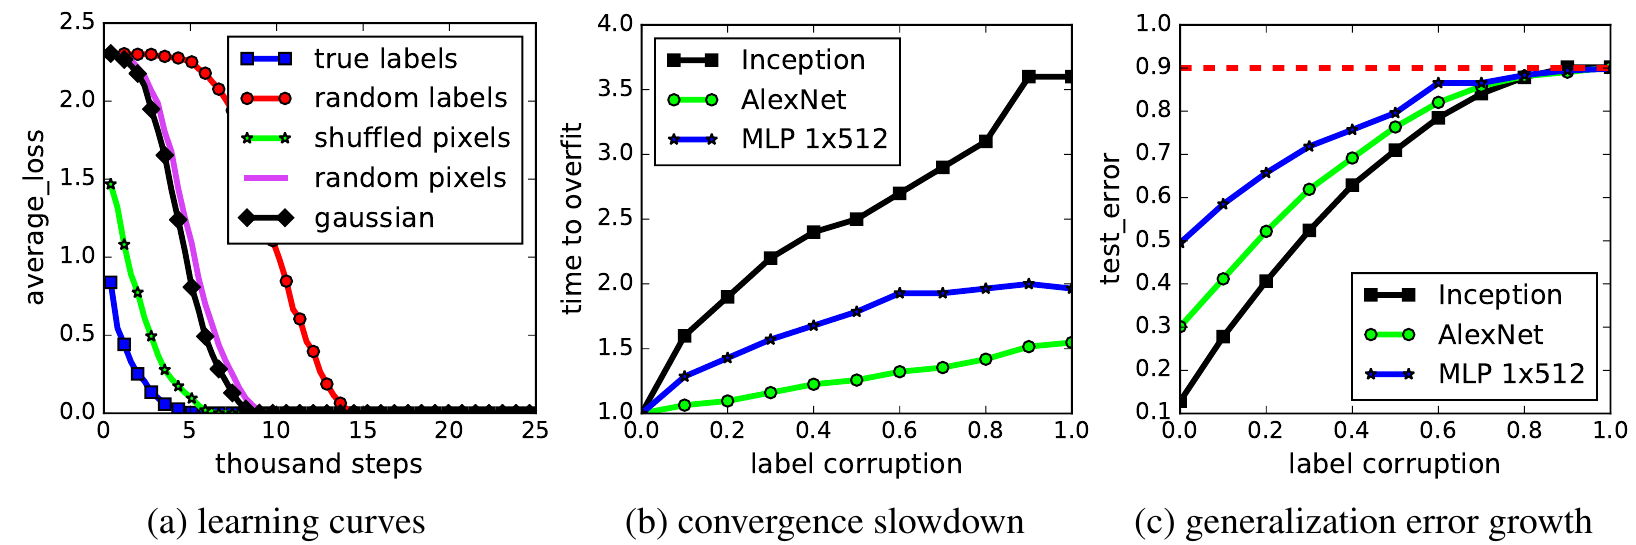
\includegraphics[width=0.84\textwidth]{figures/original_fig1.png}\\[6pt]
  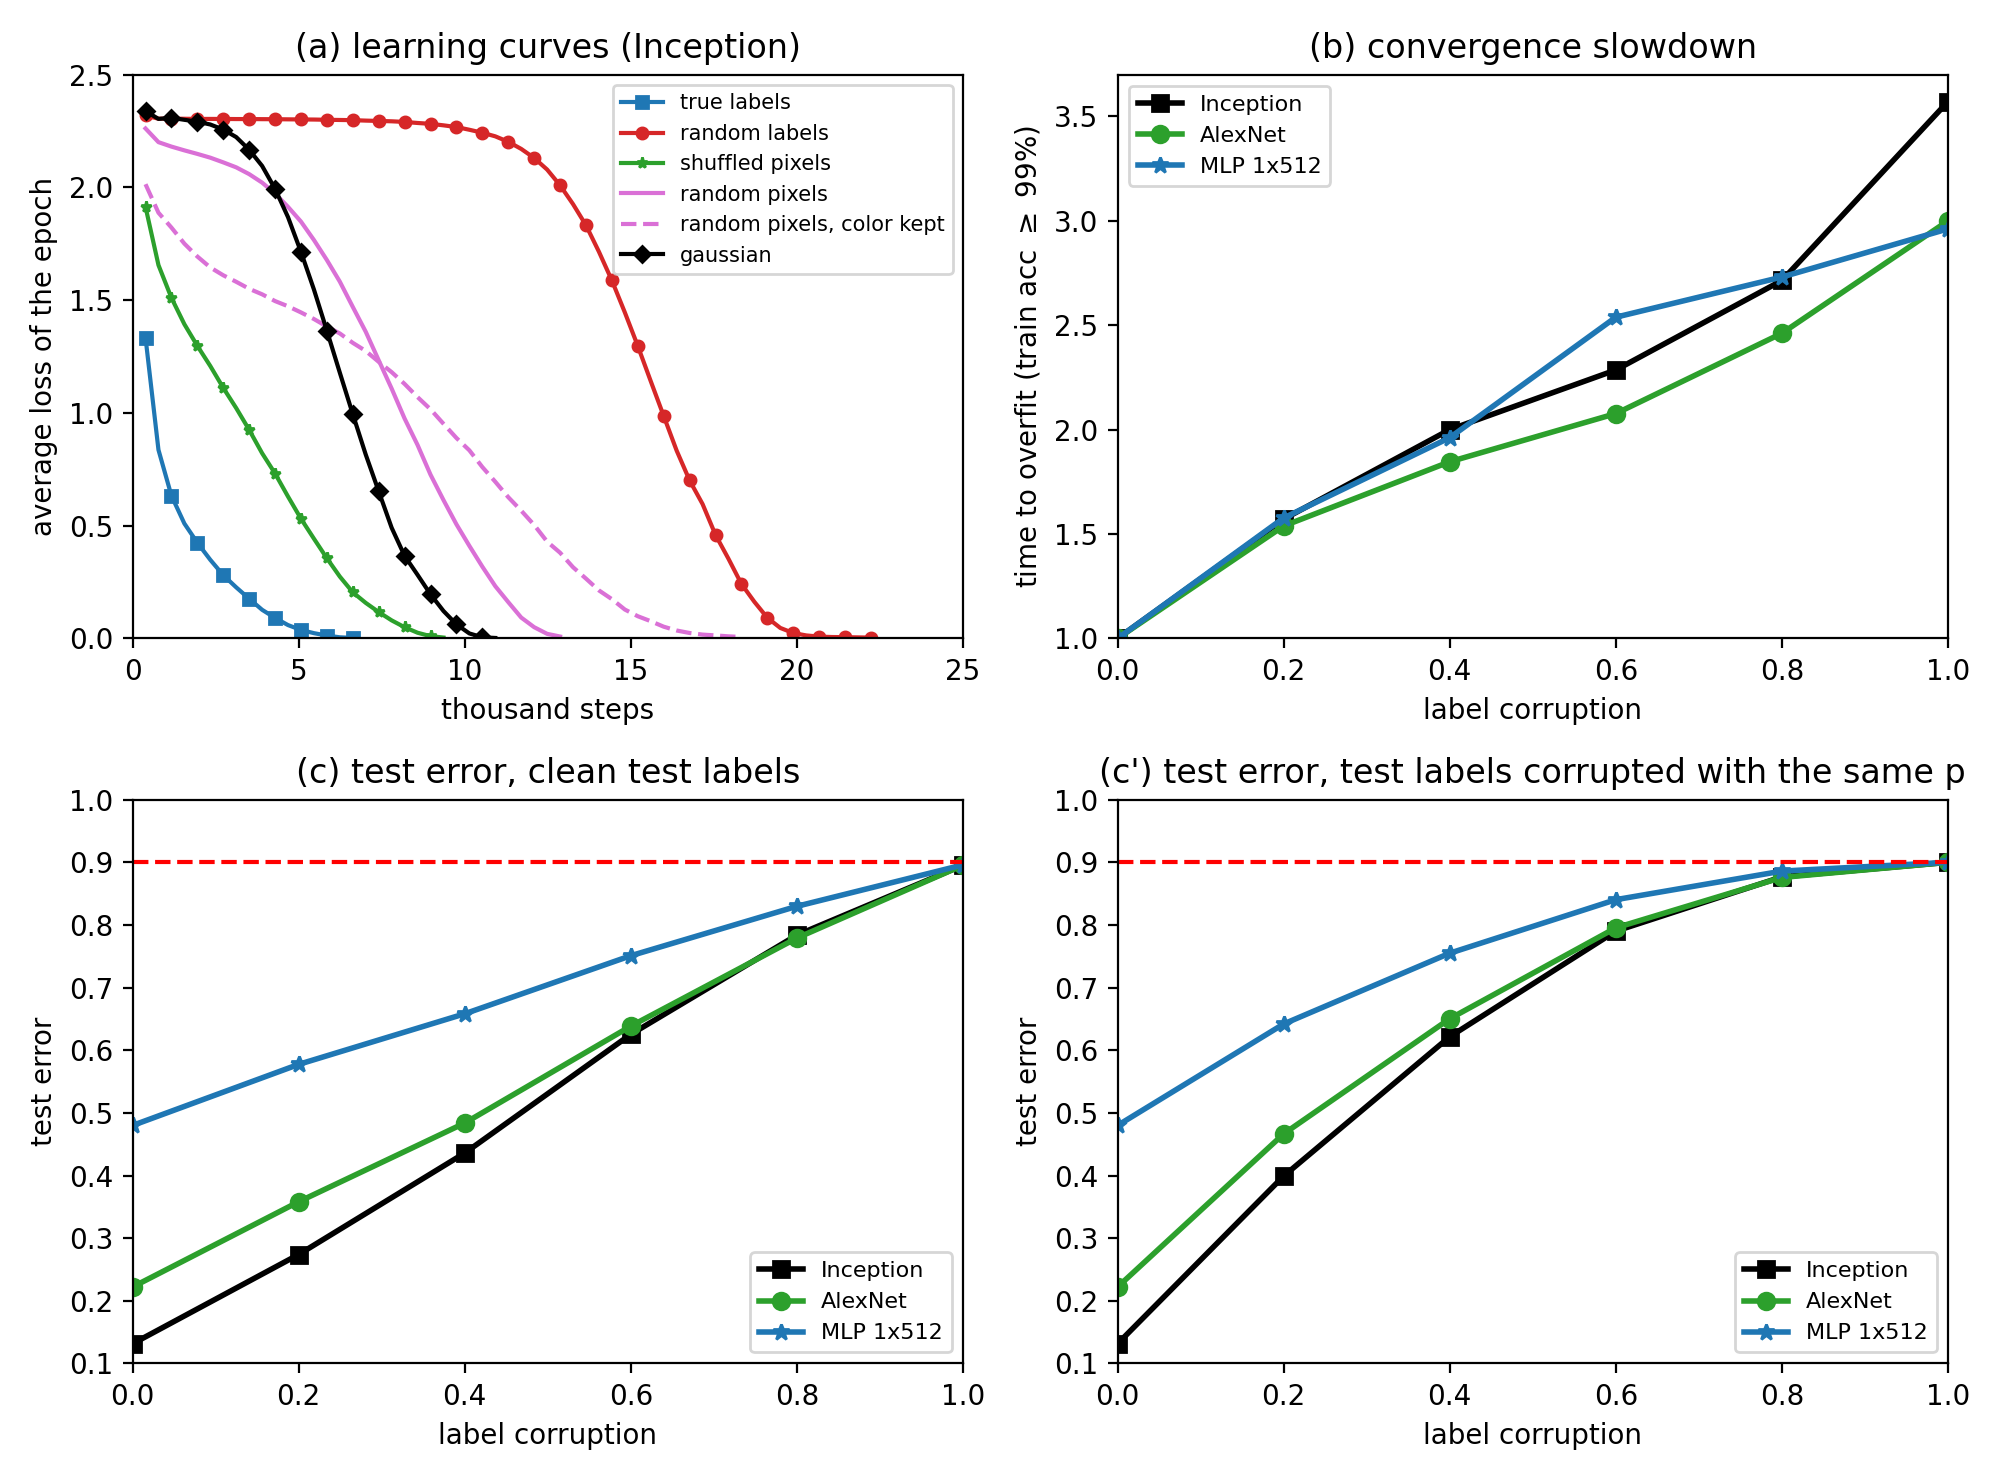
\includegraphics[width=0.68\textwidth]{figures/fig1_reproduced.png}
  \caption{Top: Figure 1 of the paper. Bottom: my reproduction. Panel (c) uses the clean test labels and panel (c$'$) uses test labels corrupted with the same $p$ as the training labels (Section~\ref{sec:mismatch}).}
  \label{fig:fig1}
\end{figure}

\subsection{Results}
In panel (a) all five settings reach 100\% training accuracy and small training loss with the same hyper-parameters, in the same order as in the paper: true labels reach 100\% training accuracy after 6{,}630 steps, then shuffled pixels (9{,}360), Gaussian noise (10{,}920), random pixels (12{,}870) and random labels (22{,}230). With random labels the loss stays at $\log 10$ for about 10{,}000 steps before it drops. In panel (b), label noise slows Inception down by at most 3.6 times, as in the paper. In panel (c), Inception's test error goes from 13\% to 90\% while its training error stays at zero. All numbers are in Table~\ref{tab:numbers}.

\begin{table}[t]\centering\small
  \begin{tabular}{@{}l c cc cccc@{}}
    \toprule
    & & \multicolumn{2}{c}{time to overfit} & \multicolumn{4}{c}{test error}\\
    \cmidrule(lr){3-4}\cmidrule(l){5-8}
    & & & & & & \multicolumn{2}{c}{mine, corrupted labels}\\
    \cmidrule(l){7-8}
    network & $p$ & paper & mine & paper & mine, clean & formula & measured\\
    \midrule
    Inception & 0.0 & 1.00 & 1.00 & 0.129 & 0.131 & 0.131 & -- \\
    & 0.2 & 1.90 & 1.57 & 0.406 & 0.274 & 0.399 & -- \\
    & 0.4 & 2.40 & 2.00 & 0.629 & 0.436 & 0.622 & -- \\
    & 0.6 & 2.70 & 2.29 & 0.785 & 0.625 & 0.790 & -- \\
    & 0.8 & 3.10 & 2.71 & 0.879 & 0.784 & 0.877 & -- \\
    & 1.0 & 3.60 & 3.57 & 0.902 & 0.895 & 0.900 & -- \\
    \addlinespace
    AlexNet & 0.0 & 1.00 & 1.00 & 0.301 & 0.222 & 0.222 & -- \\
    & 0.2 & 1.10 & 1.54 & 0.522 & 0.358 & 0.466 & -- \\
    & 0.4 & 1.23 & 1.85 & 0.692 & 0.484 & 0.650 & 0.654 \\
    & 0.6 & 1.32 & 2.08 & 0.820 & 0.639 & 0.795 & 0.798 \\
    & 0.8 & 1.42 & 2.46 & 0.881 & 0.779 & 0.876 & 0.871 \\
    & 1.0 & 1.55 & 3.00 & 0.901 & 0.895 & 0.900 & 0.900 \\
    \addlinespace
    MLP $1\times512$ & 0.0 & 1.00 & 1.00 & 0.495 & 0.480 & 0.480 & 0.480 \\
    & 0.2 & 1.43 & 1.58 & 0.657 & 0.577 & 0.642 & 0.641 \\
    & 0.4 & 1.68 & 1.96 & 0.757 & 0.658 & 0.755 & 0.757 \\
    & 0.6 & 1.93 & 2.54 & 0.865 & 0.751 & 0.840 & 0.840 \\
    & 0.8 & 1.96 & 2.73 & 0.883 & 0.830 & 0.886 & 0.886 \\
    & 1.0 & 1.96 & 2.96 & 0.898 & 0.896 & 0.900 & 0.905 \\
    \bottomrule
  \end{tabular}
  \caption{The paper against my runs. The paper's values are read from the vector graphics of its PDF (\code{extract\_paper\_fig1.py}). Time to overfit is relative to $p=0$. ``Corrupted labels'' are test labels corrupted with the same $p$ as the training labels: ``formula'' is computed from the clean accuracy (Section~\ref{sec:mismatch}), and ``measured'' is counted directly, which I only did for runs made after I added that metric.}
  \label{tab:numbers}
\end{table}

\subsection{Phases 1--3: failures and corrections}
In Phase~1 I gave the LLM the paper PDF and asked for PyTorch code that reproduces Figure~1. Checking that code against the paper and running it (Phases 2 and 3) turned up these problems:
\begin{itemize}
  \item \textbf{Parameter count.} The first small Inception had 1{,}651{,}114 parameters, 1{,}712 more than Table~1. That is exactly the number of batch-norm channels: the authors' batch norm has no scale parameter and their convolutions have no bias. With that fixed, all network sizes match Table~1 exactly. Matching AlexNet's count also pinned down details the text leaves open, such as two pooling steps down to a $7\times7$ map.
  \item \textbf{Convergence time.} The first version used 100\% training accuracy, so panel (b) had no MLP curve. I switched to 99\%.
  \item \textbf{Parallel jobs.} Four jobs at once on the laptop GPU were barely faster than one and crashed the laptop, so runs now go one at a time with a checkpoint after every epoch.
\end{itemize}
The Inception sweep was still running when I saved the Phase~3 snapshot, so I found the mismatches below after it. The random-pixels and speed checks are my own; the explanation for panel (c) came from the authors' demo in Phase~4.

\subsection{What did not match, and why}\label{sec:mismatch}
\textbf{Test error in panel (c).} On clean test labels my errors at intermediate $p$ are well below the paper's (Inception: 0.274 against 0.406 at $p=0.2$, 0.436 against 0.629 at $p=0.4$), while $p=0$ and $p=1$ agree. My code checked out: $0.9p$ of the labels change, the preprocessing follows Appendix~A, and longer training does not close the gap (the MLP uses all 100 epochs and is still lower). The answer was in the first author's demo, which corrupts the test labels with the same $p$. If $a$ is the clean test accuracy, a corrupted test label is still the true class with probability $1-0.9p$ and is any particular wrong class with probability $p/10$, independently of the network, so
\[
  \text{accuracy on corrupted labels}=a\,(1-0.9p)+(1-a)\,\frac{p}{10}.
\]
For Inception at $p=0.4$ this gives an error of 0.622 against the paper's 0.629, and the largest difference over all $p$ is 0.007. For the MLP and AlexNet I also measured it directly, and it agrees with the formula to within 0.005. So the paper's Figure~1c is consistent with corrupted test labels, not clean ones. On clean labels the test error grows roughly linearly in $p$, and corrupting the test labels as well explains the steeper curve. This is supported by the demo and numerical agreement, rather than direct access to the original training code.

\textbf{Random pixels in panel (a).} My first version permuted pixel positions but kept the three color values of each pixel together. That keeps the colors of the image, which carry class information: the loss falls right away (2.01 in the first epoch against 2.31 in the paper) and the test accuracy is still 37\%. Permuting all 2352 values gives a first-epoch loss of 2.26 and 14\% test accuracy, which matches the paper's curve, so that is my ``random pixels'' curve and the first version is dashed.

\textbf{Speed in panel (a).} My Inception is about 1.4 times slower in absolute steps (epoch loss below 0.1 after 4{,}290 steps on true labels against 3{,}130 in the paper), but the ratios to the true-label run agree: 4.5 against 4.4 for random labels, 2.3 against 2.5 for Gaussian inputs, 2.7 against 2.6 for random pixels. The batch size is not the cause, since the points in the paper's Figure~1a are 391 steps apart, one epoch at batch size 128. Neither is the initialization: with TensorFlow's default (Glorot uniform) the first-epoch loss is 1.31 instead of 1.33, while the paper has 0.84. I could not find the cause.

\textbf{Slowdown for AlexNet and the MLP in panel (b).} The ratio depends on the threshold. At 99\% Inception matches the paper, the MLP only matches at 95\% (2.15 against 1.96 at $p=1$), and AlexNet does not match at any threshold (3.0 against 1.55). The paper's AlexNet ratios are multiples of $1/31$, so its true-label run took 31 time units and its random-label run 48. If a unit is an epoch, my AlexNet needs a similar 39 epochs on random labels but only 13 on true labels. The paper's AlexNet also has 30.1\% test error at $p=0$ in Figure~1c but 23.9\% in its own Table~1 (mine has 22.2\%), so I suspect the AlexNet in Figure~1 was not trained exactly as Appendix~A describes.

\subsection{Phase 4: comparison with the authors' code}
The authors never released the code for the paper. The first author's repository \repo{pluskid/fitting-random-labels} says so and offers a small PyTorch demo with a Wide ResNet and an MLP. Like my Phase~3 code, it corrupts the labels once with a fixed seed using a uniform draw that can return the true class, uses batch size 128, and measures training accuracy on the whole training set after every epoch. The main difference is that it also corrupts the test labels. It also uses a step learning-rate schedule and $32\times32$ inputs, where I kept the paper's Appendix~A; the paper's MLP parameter count only works out for a $28\times28$ input.

Changes after the Phase~3 snapshot: a second test metric in \code{train.py} (accuracy on corrupted test labels) and panel (c$'$), because of the demo, with training unchanged; the second random-pixels version and the Glorot option, for my own diagnostics; panel (a) with one point per epoch, like the paper; and the script that reads the paper's values from its PDF. The final cleanup keeps the saved training results and adds CPU and device random-number states to new checkpoints. This affects continuation after an interruption, not the objective or the reported completed runs. The notebook reads the committed measurements by default.

\section{Critical review}

\subsection{My review}
The paper shows that standard image classifiers reach zero training error on random labels and random inputs without changing any settings, and concludes that capacity measures that ignore the data cannot explain why the same networks generalize on real data.

\textbf{Strengths.} The experiment is simple, cheap and easy to check (I reproduced every qualitative claim of Figure~1 on a laptop), and it answers one clear question. Its main value is as a negative result: it tells theory where not to look. The theorem and the linear-model section are modest, and the paper presents them that way.

\textbf{Weaknesses.}
\begin{itemize}
  \item The surprise is partly rhetorical. With about 30 weights per training image, memorizing the training set is expected, and a nearest-neighbor rule does it too. The new fact is narrower: the \emph{same recipe} that generalizes on real data also memorizes noise.
  \item ``A small constant factor'' undersells the slowdown: 3.6 times for Inception, and with random labels the loss does not move for 10{,}000 steps. That plateau shows SGD treats noise differently from signal, which the paper does not follow up.
  \item Early stopping is dismissed too quickly. With 40\% label noise my Inception had 26\% test error after 8 epochs and 44\% after memorizing the training set. The network learns the real pattern first, so early stopping does help under label noise; the paper only tests it on clean data.
  \item Section~5 does not carry over to deep networks: the minimum-norm result needs a linear model started at zero, and the section itself shows that the norm does not predict test error.
  \item There are no error bars. Every curve in Figure~1 is a single run, and so are mine.
\end{itemize}

\textbf{Possible errors and unclear points.}
\begin{itemize}
  \item Figure~1c is labeled ``test error'' but matches test labels corrupted like the training labels (Section~\ref{sec:mismatch}). The paper does not say this, and it changes the shape of the curve.
  \item ``Time to overfit'' is never defined. The plotted ratios are multiples of $1/10$, $1/31$ and $1/28$ for the three networks, so it seems to be counted in whole units, probably epochs.
  \item AlexNet has 30.1\% test error at $p=0$ in Figure~1c but 23.9\% in Table~1.
  \item ``Random labels'' and ``random pixels'' are not fully specified; the labels were only cleared up in the OpenReview discussion.
\end{itemize}

\subsection{Comparison with the OpenReview reviews}
\noindent\href{https://openreview.net/forum?id=Sy8gdB9xx}{OpenReview discussion and public reviews}.

The reviewers gave 10, 9 and 10, and the paper was accepted as an oral; the program committee called it ``groundbreaking''. Numbering the reviewers as the authors do in their reply: Reviewer~3 liked that the paper raises a good question even without answering it, and Reviewer~2 agreed with all the conclusions and only asked the authors to state that random labels come from the same label set. Reviewer~1 also gave a 10 but was more reserved, calling most results ``intuitive'', saying the authors ``do not draw a conclusion or offer a strong insight'', and asking why two networks with the same number of parameters generalize differently.

The public comments were harsher and closer to my view. Thomas Dietterich called the results ``completely unsurprising'' (replace ``neural net'' with ``decision tree''), noted that training time ``nearly tripled'' on random labels, and said early stopping has always been the real control of complexity. An anonymous commenter argued that the behavior in Section~5 comes from the zero initialization, not from SGD.

So my review shares three points with these comments: the surprise is overstated, the slowdown is not small, and Section~5 does not transfer. I also agree with Reviewer~1 that the paper diagnoses the problem without explaining it. Two of my points do not come up anywhere: the corrupted test labels behind Figure~1c, which I only found by reproducing it, and the measured benefit of early stopping under label noise. Unlike the harshest critics, I think that showing memorization with unchanged hyper-parameters on standard networks, and spelling out what that means for capacity-based bounds, was worth publishing. I would have accepted the paper, but with a score below 10.

\end{document}
